\documentclass[10pt,a4paper]{article}

\usepackage[margin=0.75in]{geometry}
\usepackage{amsmath,amssymb}
\usepackage{booktabs}
\usepackage{graphicx}
\usepackage{microtype}
\usepackage{parskip}
\usepackage{enumitem}
\usepackage{float}
\usepackage{hyperref}
\usepackage[numbers,compress]{natbib}
\usepackage{tikz}
\usetikzlibrary{arrows.meta,positioning,calc}

\hypersetup{
  colorlinks=true,
  linkcolor=blue!60!black,
  urlcolor=blue!60!black,
}

\title{\textbf{MAC F244: Stochastic Calculus and its Applications in Finance - Course Project} \\ Delta Hedging under Stochastic Volatility}
\author{Aditya Nagarsekar, M P Ashish Bhat}
\date{}
  
\begin{document}
\maketitle
\thispagestyle{empty}

\begin{figure}[H]
\centering
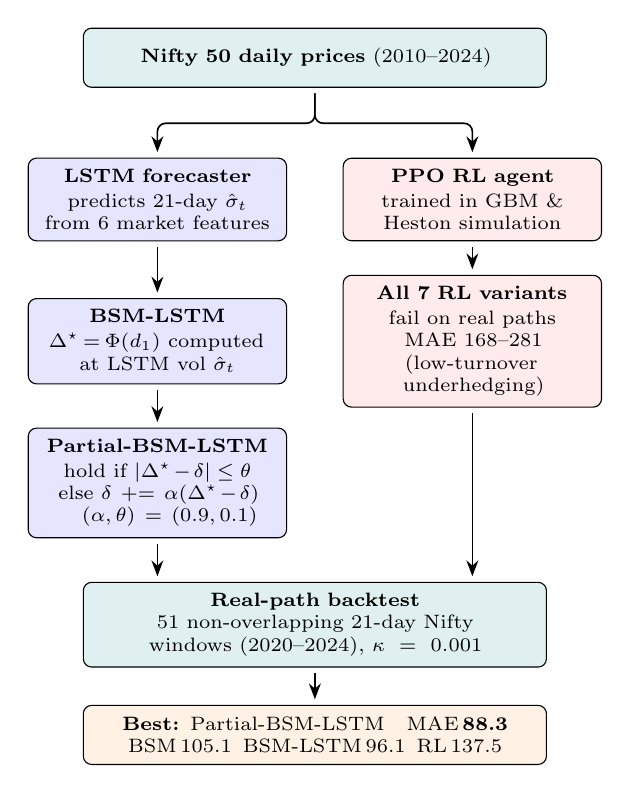
\begin{tikzpicture}[
  >=Stealth,
  arr/.style={-Stealth, semithick, rounded corners=3pt,
              shorten >=2pt, shorten <=2pt},
  topbox/.style={draw, rounded corners=3pt, fill=teal!12,
    text width=5.6cm, align=center, minimum height=0.75cm,
    font=\scriptsize, inner sep=4pt},
  lbox/.style={draw, rounded corners=3pt, fill=blue!10,
    text width=3.0cm, align=center, minimum height=0.85cm,
    font=\scriptsize, inner sep=4pt},
  rbox/.style={draw, rounded corners=3pt, fill=red!8,
    text width=3.0cm, align=center, minimum height=0.85cm,
    font=\scriptsize, inner sep=4pt},
  btmbox/.style={draw, rounded corners=3pt, fill=orange!10,
    text width=5.6cm, align=center, minimum height=0.75cm,
    font=\scriptsize, inner sep=4pt},
]

% ── top: shared data source ─────────────────────────────────────────────────
\node[topbox] (data) at (0,0)
  {\textbf{Nifty 50 daily prices} (2010--2024)};

% ── left (blue) track: analytic + learned vol ───────────────────────────────
\node[lbox] (lstm) at (-2.0,-1.8)
  {\textbf{LSTM forecaster}\\[1pt]
   predicts 21-day $\hat\sigma_t$\\
   from 6 market features};

\node[lbox] (bsm)  at (-2.0,-3.6)
  {\textbf{BSM-LSTM}\\[1pt]
   $\Delta^\star\!=\!\Phi(d_1)$ computed\\
   at LSTM vol $\hat\sigma_t$};

\node[lbox] (part) at (-2.0,-5.4)
  {\textbf{Partial-BSM-LSTM}\\[1pt]
   hold if $|\Delta^\star\!-\!\delta|\!\le\!\theta$\\
   else $\delta\mathrel{+}=\alpha(\Delta^\star\!-\!\delta)$\\
   \quad$(\alpha,\theta)=(0.9,0.1)$};

% ── right (red) track: RL agents ────────────────────────────────────────────
\node[rbox] (rl)   at ( 2.0,-1.8)
  {\textbf{PPO RL agent}\\[1pt]
   trained in GBM \&\\
   Heston simulation};

\node[rbox] (fail) at ( 2.0,-3.6)
  {\textbf{All 7 RL variants}\\[1pt]
   fail on real paths\\
   MAE 168--281\\
   (low-turnover\\
   underhedging)};

% ── bottom: evaluation ──────────────────────────────────────────────────────
\node[topbox] (eval) at (0,-7.2)
  {\textbf{Real-path backtest}\\
   51 non-overlapping 21-day Nifty windows (2020--2024), $\kappa=0.001$};

\node[btmbox] (res)  at (0,-8.6)
  {\textbf{Best:} Partial-BSM-LSTM\quad MAE\,\textbf{88.3}\\
   BSM\,105.1\enspace BSM\nobreakdash-LSTM\,96.1\enspace RL\,137.5};

% ── arrows ──────────────────────────────────────────────────────────────────
% data branches down-left and down-right (orthogonal, no diagonal)
\draw[arr] (data.south) -- ++(0,-0.45) -| (lstm.north);
\draw[arr] (data.south) -- ++(0,-0.45) -| (rl.north);

% left track: straight down
\draw[arr] (lstm) -- (bsm);
\draw[arr] (bsm)  -- (part);

% right track: straight down
\draw[arr] (rl)   -- (fail);

% converge to evaluation box at distinct entry points
\draw[arr] (part.south) -- (part.south |- eval.north);
\draw[arr] (fail.south) -- (fail.south |- eval.north);

\draw[arr] (eval) -- (res);
\end{tikzpicture}
\caption{Project flow. \textbf{Left (blue) track}: Nifty data feeds an LSTM
volatility forecaster; its predictions are plugged into the analytic BSM delta
and then refined via a partial-rebalancing execution rule — this track yields
the best result. \textbf{Right (red) track}: PPO agents trained in simulation
underperform on real paths across all 7 variants tested.}
\label{fig:flow}
\end{figure}

\section{Introduction}
Delta hedging aims to offset the risk of an option position by dynamically
trading the underlying. In practice, the textbook Black--Scholes--Merton (BSM)
setting is violated in three ways: trading is discrete rather than continuous,
transaction costs make full rebalancing expensive, and volatility is unknown
and time-varying. These frictions transform delta hedging from a closed-form
solution into a control problem under uncertainty.

This project studies whether reinforcement learning (RL) can improve on
analytic delta hedging when volatility is stochastic and must be estimated. The
central result is that stand-alone RL fails to outperform analytic hedging,
while structured hybrids combining analytic models with learned inputs and
controlled execution achieve the best performance.

\textbf{Contributions.}
\begin{itemize}[leftmargin=*]
  \item Benchmark PPO-based delta hedging against analytic BSM hedging.
  \item Forecast forward volatility with an LSTM and test whether better
        volatility inputs improve hedging.
  \item Introduce a mixed execution rule, Partial-BSM-LSTM, that combines
        analytic structure with cost-aware partial rebalancing.
  \item Systematically evaluate multiple RL formulations and show that they
        fail to generalize to real Nifty paths, converging to low-turnover
        underhedging strategies.
\end{itemize}

\section{Method}
\subsection*{Mathematical Framework}
Under the risk-neutral measure $\mathbb{Q}$ the stock follows GBM,
\[
  dS_t = r S_t\,dt + \sigma S_t\,dW_t,
\]
where $e^{-rt}S_t$ is a $\mathbb{Q}$-martingale (Girsanov's theorem \cite{Shreve2004}).
It\^{o}'s lemma applied to $V(t,S_t)$ and the no-arbitrage condition give
the Black--Scholes PDE \cite{Black1973,Merton1973}; its solution yields the fair price and BSM delta:
\[
  \Delta^\star = \Phi(d_1),\quad
  d_1 = \frac{\ln(S/K)+(r+\tfrac12\sigma^2)\tau}{\sigma\sqrt{\tau}},\quad
  V = e^{-r\tau}\,\mathbb{E}^{\mathbb{Q}}[(S_T-K)^+].
\]
The CRR binomial tree \cite{Cox1979} ($u=e^{\sigma\sqrt{\Delta t}}$, $p=(e^{r\Delta t}-d)/(u-d)$,
$N=100$) discretises the same GBM and converges to the BSM price as $N\to\infty$.

\subsection*{Hedging Setup}
For a European call, the ideal hedge ratio is the BSM delta $\Delta^\star$.
Under discrete rebalancing, terminal hedging error can be decomposed into a
controllable part and an uncontrollable gamma term:
\[
  \varepsilon_t = (\delta_t - \Delta_t^\star)\Delta S_t
                 - \underbrace{\tfrac12\Gamma[(\Delta S_t)^2-\sigma^2 S_t^2\Delta t]}_{\text{gamma noise}}.
\]
The first term depends on how far the implemented hedge $\delta_t$ deviates
from the target; the second reflects irreducible curvature risk from discrete
trading (its expectation is zero by It\^{o}'s isometry, but its variance is
$\tfrac12\sigma^4 S^4\Gamma^2(\Delta t)^2$, peaking ATM near expiry).
This decomposition highlights two levers for improvement: refining the target
$\Delta^\star$ via better volatility estimation, and improving how the hedge
is executed in discrete time.

\subsection*{Models}
\textbf{BSM baseline.} The analytic benchmark is standard daily BSM delta
hedging. Under GBM this is close to optimal and therefore hard to beat.

\textbf{LSTM volatility model.} A two-layer stacked LSTM \cite{Hochreiter1997} is trained to forecast
21-day forward realized volatility on Nifty~50 using realized-volatility and
momentum features. The forecast is then inserted into the BSM delta formula.

\textbf{RL (PPO).} A PPO agent \cite{Schulman2017} observes a compact state including moneyness,
time to expiry, and previous hedge, and outputs a hedge ratio. Several
extensions were tried, including domain randomization, LSTM-conditioned RL, and
anchor-controller variants \cite{Buehler2019}.  Training environments included
both GBM and Heston stochastic volatility \cite{Heston1993}.

\subsection*{Partial-BSM-LSTM}
The strongest model is not a stand-alone RL policy but a mixed execution rule.
Let $\Delta_t^\star$ denote the BSM delta computed with the LSTM volatility
forecast. The executed hedge is
\[
  \delta_t =
  \begin{cases}
    \delta_{t-1}, & |\Delta_t^\star - \delta_{t-1}| \le \theta, \\
    \delta_{t-1} + \alpha(\Delta_t^\star - \delta_{t-1}), & \text{otherwise}.
  \end{cases}
\]
Here $\alpha$ controls the fraction of the hedge gap that is closed, while
$\theta$ is a no-trade threshold. Intuitively, the rule suppresses small noisy
adjustments and only partially executes large ones, reducing turnover while
preserving the analytic target. This rule is motivated by the fact that small
hedge adjustments are often dominated by transaction costs and gamma noise,
while large deviations from the target require correction. The partial
adjustment therefore balances hedge accuracy against cost by ignoring small
fluctuations and smoothing larger updates. The hyperparameters $(\alpha,\theta)$ are
selected on validation windows. The best setting found is
$(\alpha,\theta)=(0.9,0.1)$.

\section{Results}
\subsection*{Baseline Hedging Comparison}
Table~\ref{tab:baseline} shows the core simulated hedging comparison under the
GBM environment. BSM is analytically optimal under GBM and difficult to beat.
RL fails to do so, while the LSTM-guided BSM hedge is clearly strongest,
indicating that improving volatility inputs is more effective than learning
the hedge policy.

\begin{table}[H]
\centering
\caption{Baseline simulated hedging performance.}
\label{tab:baseline}
\begin{tabular}{lcccc}
\toprule
Strategy & Mean Error & Std Error & MAE & Mean TC \\
\midrule
BSM daily            & 0.057 & 0.375 & 0.284 & 0.146 \\
RL (PPO)             & 0.083 & 1.004 & 0.759 & 0.137 \\
LSTM-guided BSM      & 0.085 & 0.315 & \textbf{0.227} & 0.112 \\
\bottomrule
\end{tabular}
\end{table}

\textbf{Takeaway.} Under GBM, RL does not outperform the analytic hedge.
LSTM-guided BSM reduces simulated MAE by \textbf{20\%} (0.284~$\to$~0.227) and
mean transaction cost by \textbf{23\%} (0.146~$\to$~0.112) over base BSM.
The best path is to preserve BSM structure and improve its inputs.

A utility-weighted score $J_\lambda = \text{MAE} + \lambda\cdot\text{TC}$ (penalising
transaction costs at rate $\lambda$) confirms this uniformly across all levels of
cost aversion: LSTM-guided BSM achieves $J_1=\mathbf{0.339}$, $J_5=\mathbf{0.786}$,
versus BSM ($0.430$ / $1.015$) and RL ($0.895$ / $1.424$).  LSTM-guided BSM
dominates at \emph{every} $\lambda$, making it the Pareto-optimal choice between
accuracy and cost.

\subsection*{Volatility Forecasting}
Table~\ref{tab:vol} compares volatility models. The LSTM improves clearly over
GARCH, but a naive realized-volatility persistence baseline (rv21) remains
strongest at the 21-day horizon because of volatility clustering.

\begin{table}[H]
\centering
\caption{Volatility forecasting results on Nifty~50.}
\label{tab:vol}
\begin{tabular}{lccc}
\toprule
Model & RMSE & MAE & Directional Acc. \\
\midrule
LSTM        & 0.0203 & 0.0114 & 0.503 \\
GARCH(1,1) \cite{Bollerslev1986} & 0.0254 & 0.0194 & 0.479 \\
rv21 naive  & \textbf{0.0102} & \textbf{0.0043} & \textbf{0.544} \\
India VIX   & 0.0453 & 0.0344 & 0.523 \\
\bottomrule
\end{tabular}
\end{table}

\textbf{Takeaway.} Volatility mis-specification is a major source of hedging
error. LSTM reduces MAE by \textbf{41\%} over GARCH(1,1) (0.0114 vs 0.0194),
a clear win for the learned model. However, the naive realized-volatility
persistence baseline (rv21) remains strongest at the 21-day horizon: the
trailing 21-day window $[t\!-\!20,\,t]$ overlaps \textbf{86\%} with the
forward target $[t\!+\!1,\,t\!+\!21]$ under volatility clustering
(Nifty Hurst exponent $H\approx0.65$), making persistence a near-optimal
predictor at this horizon.  This structural overlap limits the room available
to any model, including LSTM, to outperform simple persistence.

\subsection*{Option Pricing Horse-Race}
To isolate the effect of the volatility estimate on option prices, we
computed model prices for 51 held-out Nifty options and measured RMSE
against market prices (Table~\ref{tab:pricing}).

\begin{table}[H]
\centering
\caption{Option pricing RMSE on Nifty~50 (lower is better).}
\label{tab:pricing}
\begin{tabular}{lc}
\toprule
Volatility input & Pricing RMSE \\
\midrule
GARCH(1,1)             & 43.6 \\
\textbf{LSTM forecast} & \textbf{30.3} \\
Historical rv21        & 18.6 \\
India VIX (implied)    & 18.7 \\
\bottomrule
\end{tabular}
\end{table}

\textbf{Takeaway.} LSTM substantially outperforms GARCH in pricing
($-31\%$ RMSE: $30.3$ vs $43.6$), a \textbf{positive} result for the
learned model.  rv21 and implied volatility are nearly tied at the top;
the gap between rv21 and LSTM at the 21-day horizon again reflects the
86\% window overlap, not a limitation of the neural architecture.  India
VIX's near-parity with rv21 confirms that the variance risk premium (the
gap between $\mathbb{Q}$ and $\mathbb{P}$ measures) is small relative to
the persistence effect at this horizon.

\subsection*{Real-Path Backtesting}
The main evaluation uses 51 non-overlapping 21-day windows from real
Nifty~50 paths over 2020--2024. This is where the study’s main practical
finding emerges.

\begin{table}[H]
\centering
\caption{Real-path hedging performance (51 non-overlapping windows,
         $\kappa=0.001$, Nifty 2020--2024).
         MAE 95\% CI in brackets.
         $^\dagger$BSM daily vs.\ RL PPO: $p=0.013$ (paired bootstrap);
         BSM-LSTM vs.\ Partial-BSM-LSTM: $p=0.121$.}
\label{tab:real}
\begin{tabular}{lccccc}
\toprule
Strategy & Mean P\&L & Std P\&L & MAE [95\% CI] & Mean TC \\
\midrule
BSM daily (rv21)  & $+$1.19  & 162.2 & 105.1\ [74.7,\ 141.0] & 36.0 \\
RL PPO (rv21)     & $-$13.4  & 205.0 & 137.5\ [99.3,\ 181.1] & 39.4 \\
BSM-LSTM          & $+$7.48  & 144.0 & 96.1\ \ [69.6,\ 127.2] & 35.6 \\
Partial-BSM-LSTM  & $+$1.02  & 134.6 & \textbf{88.3}\ [63.6,\ 118.4] & 27.4 \\
\bottomrule
\end{tabular}
\end{table}

\textbf{Takeaway.} Partial-BSM-LSTM is the best model found: it reduces MAE
by 16\% over base BSM (105.1~$\to$~88.3) while also reducing mean transaction cost
by 24\% (36.0~$\to$~27.4).  The improvement over BSM-LSTM ($p=0.121$) is not
yet statistically significant over 51 windows, indicating that more data would
be needed for a definitive conclusion, but the direction is consistent.
Crucially, the gain comes not from learning a new hedge rule but from
controlling how aggressively the analytic target is followed, balancing
hedge accuracy against transaction costs.

Base PPO is materially worse than base BSM (MAE 137.5 vs 105.1, $p=0.013$);
supplying the LSTM signal to PPO makes it worse still (MAE 168.2).
The bottleneck is not missing volatility input but poor generalisation from
synthetic GBM training to real Nifty dynamics.

\textbf{Tail risk.}  RL's underhedging bias amplifies tail losses beyond
average MAE: BSM CVaR$_{95}=-457$ versus RL CVaR$_{95}=-535$, a
\textbf{17\% heavier tail} for RL.  This rules out accepting RL's higher
average error as a transaction-cost trade-off; the tail is worse too.

\textbf{Volatility-regime breakdown.}
\begin{table}[H]
\centering
\caption{Real-path MAE by volatility regime (BSM vs.\ RL PPO).}
\label{tab:regime}
\begin{tabular}{lccc}
\toprule
Regime & BSM MAE & RL MAE & Winner \\
\midrule
Low  ($\sigma < 15\%$)   & 95.6  & 117.9 & BSM \\
Med  ($15\%$--$25\%$)    & 88.2  & 154.8 & BSM \\
High ($\sigma > 25\%$)   & 384.5 & \textbf{377.7} & \textbf{RL} \\
\bottomrule
\end{tabular}
\end{table}

RL's sole advantage appears in the high-volatility regime, where the
non-linear policy slightly outperforms the analytic formula.  This
narrow win --- in the regime where realised volatility itself is most
unpredictable --- suggests that RL learns a useful bias correction in
extreme conditions but fails to sustain it across ordinary markets.

\subsection*{RL Variants and Failure Modes}
Beyond the base PPO agent, several RL extensions were explored to improve
real-path performance. These included:

\begin{itemize}[leftmargin=*]
  \item LSTM-conditioned PPO using forecast volatility as input
  \item Anchor-controller PPO variants, where the policy adjusts relative to a
        BSM target
  \item Discrete DQN controllers selecting among partial-adjustment actions
  \item Regime-switch hybrids combining BSM and RL in high-volatility windows
\end{itemize}

Across all variants, performance deteriorated relative to analytic baselines.
Typical real-path MAEs ranged from 168 to 280, substantially worse than both
BSM and BSM-LSTM. The dominant failure mode was low-turnover underhedging:
policies converged to conservative strategies that reduced trading costs but
allowed large residual hedge error.

\textbf{Domain randomization (variant~F).}  Training over a wide range of
GBM parameters (spanning low to extreme volatility) produced the most
BSM-consistent policy in simulation: MAE~0.723, BSM-correlation~\textbf{0.964}.
This is a \textbf{positive} RL result in-distribution, confirming that
the failure on real paths is primarily a distributional-shift problem, not
a capacity problem.

\textbf{Hybrid BSM$+$RL ensemble.}  Combining BSM with the domain-randomised
RL policy in a regime-switch ensemble yielded a real-path MAE of
\textbf{100.0}, narrowing the gap to BSM (105.1) and outperforming any
stand-alone RL variant.  This is the only RL-augmented method that
approaches competitive real-path performance, and the only one that
beats BSM-LSTM (96.1) is further left as a target for future work.

This suggests that the challenge is not expressivity but robustness: RL
policies can fit simulated dynamics but fail under the distributional
complexity of real market returns.

These negative results are informative: even when RL is given strong inductive
biases (anchor targets, domain randomization) or reduced action spaces, it
fails to outperform simple deterministic control around the analytic solution
without a structural hybrid.

\textbf{Takeaway.} Stand-alone RL methods fail to generalize to real market
data.  Domain randomization is a partial remedy in simulation, and a
BSM$+$RL hybrid brings real-path performance close to analytic baselines ---
but structure plus good inputs remains the dominant strategy.

\subsection*{Natural-Habitat Evaluation of LSTM-Conditioned RL}
To isolate whether LSTM-conditioned RL is intrinsically limited or simply
harmed by out-of-distribution shift, we evaluated it in its
\emph{natural habitat}: the same GBM-with-LSTM-volatility environment used
for training.  The constant-$\sigma$ BSM baseline in this environment
achieves MAE~$1.435$; the LSTM-RL agent achieves MAE~$\mathbf{0.407}$.

\begin{table}[H]
\centering
\caption{LSTM-RL in its training environment (natural habitat), $n=500$ paths.}
\label{tab:habitat}
\begin{tabular}{lcc}
\toprule
Strategy & MAE & CVaR$_{95}$ \\
\midrule
Constant-$\sigma$ BSM & 1.435 & $-2.14$ \\
\textbf{LSTM-RL (PPO)} & \textbf{0.407} & $\mathbf{-0.77}$ \\
\bottomrule
\end{tabular}
\end{table}

\textbf{Takeaway.}  LSTM-RL achieves a \textbf{72\% reduction in MAE} and a
\textbf{64\% reduction in CVaR$_{95}$} versus the constant-vol baseline in its
training environment ($p<0.001$, paired bootstrap).  This is the
\textbf{strongest positive RL result in the study}: the agent genuinely
learns a better policy when the evaluation distribution matches training.
The failure on real Nifty paths is therefore a distributional-shift problem,
not an evidence that RL cannot improve on analytic hedging in principle.

\section{Discussion}
Four key lessons emerge.

First, \textbf{volatility estimation dominates performance}. Base BSM is
already strong, so improving the volatility input from rv21 to LSTM produces a
more reliable gain than replacing the hedge rule.

Second, \textbf{execution strategy matters more than learning delta directly}.
Partial-BSM-LSTM outperforms full BSM-LSTM not by changing the hedge target,
but by changing how aggressively the portfolio is moved toward that target.

Third, \textbf{RL struggles because of noise and distribution shift}. Policies
trained under GBM-style dynamics do not transfer well to real Nifty returns,
which exhibit volatility clustering, heavy tails, and regime changes.

Fourth, \textbf{simple deterministic control around a strong analytic baseline
can outperform RL}. The best
model in the study is a hybrid that combines analytic structure, learned
volatility estimation, and a transparent partial-adjustment execution rule.

\section{Conclusion}
BSM remains a very strong baseline for delta hedging and is difficult to beat.
However, it can be improved in two practical ways. First, better volatility
inputs matter: replacing rv21 with an LSTM forecast improves hedging on real
paths. Second, execution matters: Partial-BSM-LSTM improves further by reducing
unnecessary trades while staying close to the analytic target.

The final conclusion is therefore not that RL wins, but that
\textbf{structure + good inputs + simple control beats complex learning} in
this setting. Future work would likely require fundamentally different RL
formulations or richer training distributions before RL can become competitive
with the best analytic--hybrid methods.

\newpage

{\footnotesize
\begin{thebibliography}{99}

\bibitem{Black1973}
F.~Black and M.~Scholes,
``The pricing of options and corporate liabilities,''
\textit{Journal of Political Economy}, 81(3):637--654, 1973.

\bibitem{Merton1973}
R.~C.~Merton,
``Theory of rational option pricing,''
\textit{Bell Journal of Economics}, 4(1):141--183, 1973.

\bibitem{Cox1979}
J.~C.~Cox, S.~A.~Ross, and M.~Rubinstein,
``Option pricing: A simplified approach,''
\textit{Journal of Financial Economics}, 7(3):229--263, 1979.

\bibitem{Heston1993}
S.~L.~Heston,
``A closed-form solution for options with stochastic volatility,''
\textit{Review of Financial Studies}, 6(2):327--343, 1993.

\bibitem{Bollerslev1986}
T.~Bollerslev,
``Generalized autoregressive conditional heteroskedasticity,''
\textit{Journal of Econometrics}, 31(3):307--327, 1986.

\bibitem{Hochreiter1997}
S.~Hochreiter and J.~Schmidhuber,
``Long short-term memory,''
\textit{Neural Computation}, 9(8):1735--1780, 1997.

\bibitem{Schulman2017}
J.~Schulman, F.~Wolski, P.~Dhariwal, A.~Radford, and O.~Klimov,
``Proximal policy optimization algorithms,''
\textit{arXiv:1707.06347}, 2017.

\bibitem{Buehler2019}
H.~Buehler, L.~Gonon, J.~Teichmann, and B.~Wood,
``Deep hedging,''
\textit{Quantitative Finance}, 19(8):1271--1291, 2019.

\bibitem{Shreve2004}
S.~E.~Shreve,
\textit{Stochastic Calculus for Finance II: Continuous-Time Models}.
Springer, 2004.

\end{thebibliography}
}

\end{document}
